\subsubsection{Decision tree classifiers}
	The simplest, and perhaps, widely known classifiers are based around the a tree structure. 
	These are often used within the datamining discipline in order to create a predictive model based upon some preexisting data. T
	The predictive model can then be used on new never seen before data in order to classify it. 
	
	\bigskip\noindent
	One example of this could the rating of wine quality.
	Given a dataset(Resource: \cite{mining:datasetexample}) of preexisting knowledge, which include known attributes of a set of wines and the accompanying classification. A Decision tree may be create in order to generalize the knownledge within the dataset to something usefull on other example. 
	
	\begin{figure}[H]%
		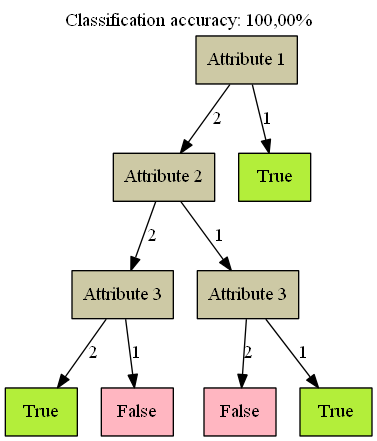
\includegraphics[width=\columnwidth]{images/TrivialDecisionTree.png}%
		\caption{Example decision tree from TDT4171}%
		\label{fig:decisiontree}%
	\end{figure}
